\documentclass[../structural_economics_book.tex]{subfiles}
\begin{document}
\ifSubfilesClassLoaded{\setcounter{chapter}{23}}{}
\chapter{Hegemony and Counter-Hegemony}\label{ch:24}
\chaptersubtitle{When the Dominated Accept the Matrix, and When They Don't}
\begin{quote}
\textit{``La crisi consiste appunto nel fatto che il vecchio muore e il nuovo non pu\`{o} nascere: in questo interregno si verificano i fenomeni morbosi pi\`{u} svariati.''}\\[0.3em]
\textnormal{[``The crisis consists precisely in the fact that the old is dying and the new cannot be born; in this interregnum a great variety of morbid symptoms appear.'']}\\
\hfill --- Antonio Gramsci, \textit{Quaderni del carcere}, Q3 \S34 (1930)
% TODO-VERIFY: page in the Gerratana critical edition (Einaudi, 1975), vol. 1; English per Hoare & Nowell Smith (1971), p. 276. The popular "monsters" version is not Gramsci's wording.
\end{quote}
\nocite{gramsci1975quaderni}

\vspace{1em}

Part~VII opens where Parts~I--VI left a question unanswered: if the current $W$ is far from $W^{CE}$, and if structural reform would make nearly everyone better off (the Structural Welfare Theorem, Chapter~12), why does the structure persist?

The answer from Chapter~14 is political: coalitions block structural change that threatens their power. But this answer is incomplete. It explains why the powerful resist change. It does not explain why the powerless \textit{accept} the structure --- why the indigenous woman in Potos\'{i} does not demand the operators that would raise her $\pi_I$ from $10^{-5}$ to something closer to $1/N$.

The answer is hegemony: the process by which the dominant coalition's preferred $W$ becomes the \textit{accepted} $W$ --- not through coercion but through the formation of preferences that regard the structure as natural, inevitable, or even desirable. In this book's notation: hegemony is the steady state of the formation model (Chapter~10) in which the $W^I$-shaped preferences of the dominated classes are calibrated to accept the $W^P$-determined allocation.

Counter-hegemony is the disruption: a change in $W^I$ that produces new preferences, new demands, new coalitions, and ultimately a new $W$. This chapter formalizes both.


%% =====================================================================
\section{Hegemony as a Structural Equilibrium}
\label{ch24:sec:hegemony}
%% =====================================================================

\subsection{Gramsci's Concept, Formalized}

\begin{definition}[Hegemony]\label{ch24:def:hegemony}
A weight matrix $W$ is \textbf{hegemonic} if it satisfies three conditions simultaneously:
\begin{enumerate}
\item \textbf{Power concentration}: $\Neff(\boldsymbol{\pi}^P)$ is well below $N$ (equivalently, $\Var(\boldsymbol{\pi}^P)$ is well above 0; Chapter~6): the structure benefits some agents substantially more than others. ($\Var > 0$ alone holds for almost every $W$ and would not discriminate.)
\item \textbf{Consent}: the steady-state preferences $\boldsymbol{\theta}^*(W^I)$ evaluate the allocation $\x^*(W, \boldsymbol{\theta}^*)$ favorably: $U_i(x_i^*, \theta_i^*) \geq U_i(x_i', \theta_i^*)$ for all feasible $x_i'$ (each agent is satisfied given her preferences).
\item \textbf{Formation alignment}: the information network $W^I$ is controlled (directly or indirectly) by the coalition that benefits from $W$: on a common node set of agents or groups, the agents with high $\pi^P_i$ also have high $\pi^I_i$ (a positive rank correlation between $\boldsymbol{\pi}^I$ and $\boldsymbol{\pi}^P$; exact proportionality would be a knife-edge case).
\end{enumerate}
Condition~2 formalizes consent only. Gramsci's hegemony is ``consent armoured by coercion'': the state combines political society (coercion) with civil society (consent). This chapter models the consent half; coercion enters only as the outside option that the dominant coalition holds in reserve.
\end{definition}

\begin{definition}[Hegemonic Equilibrium]\label{ch24:thm:hegemony}
A \textbf{hegemonic equilibrium} is a structural equilibrium (Definition~\ref{ch13:def:structural_eq}) with the additional property that the formation channel ($W^I$) \textit{stabilizes} the power structure ($W^P$) by producing preferences that consent to it.

Formally: a hegemonic equilibrium is a fixed point $(W^*, \boldsymbol{\theta}^*, \x^*)$ of the co-evolutionary system where:
\begin{equation}\label{ch24:eq:hegemony}
\boldsymbol{\theta}^* = T(\boldsymbol{\theta}^*; W^*), \quad \x^* = h(\boldsymbol{\pi}(W^*), \boldsymbol{\theta}^*), \quad W^* = \mathcal{E}(W^*; \x^*),
\end{equation}
AND the three conditions of Definition~\ref{ch24:def:hegemony} hold at $(W^*, \boldsymbol{\theta}^*, \x^*)$; in particular, no agent, given her preferences $\theta_i^*$, prefers a feasible alternative allocation, so none demands a change in $W$.

This definition asserts no existence result; whether such fixed points exist depends on the formation map $T$, the bargaining map $h$ and the network evolution map $\mathcal{E}$ (Chapter~13, Definition~\ref{ch13:thm:coevolution}). It is the Satisfaction Paradox (Proposition~\ref{ch12:thm:paradox}) with a political interpretation: the dominated classes do not demand structural change because their $W^I$-formed preferences are calibrated to the $W^P$-determined returns. The hegemony is self-reproducing.
\end{definition}

\begin{intuition}[Why hegemony is stable]
Three reinforcing loops:

\textbf{Loop 1 (Production)}: $W^P$ determines the allocation $\x^*$ through the bargaining equilibrium. The dominated receive less, but their sectors are structurally peripheral (low $\pi_i$), so there is no economic lever for change.

\textbf{Loop 2 (Information)}: $W^I$ shows the dominated their own group's returns (assortative mixing, Chapter~18). They observe low returns and form low aspirations ($\theta^*_{\text{disadv}} < \theta^*_{\text{adv}}$, Proposition~\ref{ch18:thm:attribute_trap}). Low aspirations produce low investment, low returns, confirming the signal.

\textbf{Loop 3 (Solidarity)}: $W^U$ is assortative by the same groups. The dominated care about their own group, not about the advantaged group. Cross-group solidarity is low ($\lambda^U \approx 0.2$, Chapter~22). The dominated do not form cross-class coalitions because they do not identify with the advantaged class's interests.

Hegemony is the triple alignment of loops 1, 2, and 3: the same groups are peripheral in $W^P$, informationally isolated in $W^I$, and solidaristically self-contained in $W^U$. The alignment IS the hegemony. Breaking it requires disrupting at least one loop.
\end{intuition}


\subsection{The Cost of Maintaining Hegemony}

\begin{definition}[Hegemony Maintenance Cost]\label{ch24:prop:maintenance}
Maintaining hegemony requires the dominant coalition to keep the consensus $b^* = (\boldsymbol{\pi}^I)'\bb^{(0)}$ at the target belief $b_T$ (``the structure is natural/efficient'') against the drift created by independent outlets. Model the per-period cost as
\begin{equation}\label{ch24:eq:maintenance}
C_H = \mu_H \cdot \sum_{j \notin S_H} \pi^I_j\,|b_T - b^{(0)}_j| \cdot \bigl(1 - \lambda_2(W^I)\bigr),
\end{equation}
where $S_H$ is the set of outlets the coalition already controls, $b^{(0)}_j$ is outlet $j$'s belief absent manipulation, and $\mu_H > 0$ is a cost scale. The factor $1 - \lambda_2(W^I)$ comes from the corrected manipulation cost of Chapter~8: by the perturbation lemma (Lemma~\ref{ch06:lem:perturbation}), $\boldsymbol{\pi}^I$ is cheapest to move when $\lambda_2$ is close to $+1$, i.e.\ when $W^I$ is weakly coupled.
\end{definition}

Two different properties of $W^I$ matter, and they must not be confused:
\begin{itemize}
\item \textbf{Concentration} ($\Neff^I$ small). When a few outlets the coalition controls hold most of $\boldsymbol{\pi}^I$, the sum in \eqref{ch24:eq:maintenance} is small: the coalition owns the consensus and barely needs to manipulate. As $\Neff^I$ rises, more independent weight must be countered and $C_H$ rises. A hub that everyone listens to has a \emph{large} spectral gap (Proposition~\ref{ch06:prop:gap-power-independent}), so concentration is measured by $\Neff^I$, not by $\Gamma^I$.
\item \textbf{Weak coupling} ($1-\lambda_2$ small). When $W^I$ splits into weakly connected blocks, the consensus is fragile: it is cheap for \emph{anyone}, the coalition or its challengers, to move it.
\end{itemize}

\begin{example}[Bolivia's Hegemonic Transitions \illustrative]\label{ch24:ex:bolivia_hegemony}
\begin{center}
\begin{tabular}{llcl}
\toprule
Period & Hegemonic structure & $N_{\text{eff}}^I$ & Stability \\
\midrule
Pre-1952 & Tin-mining oligarchy & $\approx 1.5$ & Stable (few media) \\
1952--1964 & MNR revolutionary state & $\approx 2.0$ & Moderately stable \\
1964--1982 & Military governments & $\approx 1.8$ & Coercion-dependent \\
1982--1985 & UDP government, hyperinflation & --- & No stable hegemony \\
1985--2003 & Neoliberal consensus & $\approx 2.5$ & Stable, then collapsed \\
2006--2019 & MAS/indigenous hegemony & $\approx 3.0$--$3.4$ & Fragile (social media) \\
2019-- & Contested & $\approx 3.5$ & No hegemony \\
\bottomrule
\end{tabular}
\end{center}

The trend: $N_{\text{eff}}^I$ has been increasing (from 1.5 to 3.5 over 70 years). On the reading of Definition~\ref{ch24:prop:maintenance}, each increase made the existing hegemony more expensive to maintain. The neoliberal consensus (1985--2003) collapsed after social movements (the Water War 2000, Gas War 2003) generated alternative $W^I$ channels that broke the information monopoly. The MAS hegemony (2006--2019) was already fragile at $N_{\text{eff}}^I \approx 3.0$--$3.4$ (the end-of-period value 3.4 is Chapter~17's, on four media ecosystems; Example~\ref{ch17:ex:bolivia_neff}); new digital channels contributed to destabilizing it in 2019. Whether digital media raise or lower $\Neff^I$ in the long run depends on the balance between new channels and algorithmic concentration within platforms (Chapter~27).
\end{example}


%% =====================================================================
\section{Counter-Hegemony as $\Delta W^I$}
\label{ch24:sec:counter}
%% =====================================================================

\begin{definition}[Counter-Hegemonic Movement]\label{ch24:def:counter}
A \textbf{counter-hegemonic movement} is a coalition $S$ of dominated agents that implements $\Delta W^I$ --- a change in the information network that disrupts the formation channel supporting the current hegemony. The movement creates alternative $W^I$ edges: new media, new narratives, new reference groups, new signals that show the dominated a different set of returns.
\end{definition}

With the linear formation rule of Chapter~10, $\theta_{t+1} = \rho\theta_t + \mu(\cdot)$, the steady state is unique, so there is no basin boundary to cross and no threshold. A threshold needs a nonlinearity. The simplest one is \emph{conformity}: the return an agent observes from acting on the alternative view rises with the share of her reference group already acting on it. Let $\theta_t \in \R$ index the intensity of counter-hegemonic preference in the dominated group ($\theta \approx 0$: consent; $\theta \approx 1$: the alternative view), and let
\begin{equation}\label{ch24:eq:counter_model}
\theta_{t+1} = \rho\,\theta_t + (1-\rho)\bigl[g(\theta_t) + s\bigr], \qquad g(\theta) = \frac{1}{1 + e^{-\beta(\theta - 1/2)}},
\end{equation}
where $g$ is the conformity response and $s \ge 0$ is the persistent counter-hegemonic signal delivered by the new $W^I$ edges, scaled so that $(1-\rho)s = \mu\,\|\Delta(W^I\mathbf{r})\|$.

\begin{proposition}[Counter-Hegemony Threshold and Saddle-Node]\label{ch24:thm:counter}
In model \eqref{ch24:eq:counter_model} with $\beta > 4$ and $0 < \rho < 1$:
\begin{enumerate}
\item For $s = 0$ there are three fixed points $\theta_h < \tfrac12 < \theta_c$ with $\theta_c = 1 - \theta_h$. The outer two (hegemonic and counter-hegemonic) are stable; the middle one, $\theta_u = \tfrac12$, is unstable and is the separatrix. A one-time shock moves the system to the counter-hegemonic equilibrium iff it pushes $\theta$ above $\theta_u$.
\item As the persistent signal $s$ rises, $\theta_h$ and the separatrix move toward each other and merge at $s^*$, defined by $g'(\theta) = 1$, $\theta < \tfrac12$ and $\theta = g(\theta) + s^*$ (a \textbf{saddle-node bifurcation}). For $s > s^*$ the hegemonic equilibrium no longer exists and $\theta$ converges to the counter-hegemonic one from every initial condition. The collapse condition is therefore
\begin{equation}\label{ch24:eq:counter_condition}
\mu\,\|\Delta(W^I\mathbf{r})\| > (1-\rho)\,s^*.
\end{equation}
\end{enumerate}
For $\beta = 10$, $\rho = 0.85$: $\theta_h = 0.007$, $\theta_u = 0.5$, $\theta_c = 0.993$ and $s^* = 0.181$; an impulse to $\theta = 0.457$ returns to $\theta_h$, an impulse to $0.557$ goes to $\theta_c$ (\texttt{code/ch24.py}).
\end{proposition}
\begin{proof}
Write $F(\theta) = \rho\theta + (1-\rho)[g(\theta) + s]$. Fixed points of $F$ solve $h(\theta) = -s$, where $h(\theta) := g(\theta) - \theta$. Since $g' > 0$, $F'(\theta) = \rho + (1-\rho)g'(\theta) > 0$, so $F$ is strictly increasing, and a fixed point is stable iff $F' < 1$ iff $g' < 1$ (no oscillatory instability is possible).

\emph{Shape of $h$.} $g'(\theta) = \beta g(1-g)$ increases on $(-\infty,\tfrac12)$, decreases on $(\tfrac12,\infty)$, has maximum $\beta/4 > 1$ at $\tfrac12$ and tends to $0$ at $\pm\infty$. Hence $g' = 1$ at exactly two points $a < \tfrac12 < b$, and $h' = g' - 1$ is negative on $(-\infty,a)$, positive on $(a,b)$, negative on $(b,\infty)$. Symmetry of the logistic, $g(1-\theta) = 1 - g(\theta)$, gives $h(1-\theta) = -h(\theta)$, so $b = 1-a$, $h(\tfrac12) = 0$ and $h(b) = -h(a)$. Since $h$ is increasing on $(a,b) \ni \tfrac12$, $h(a) < 0 < h(b)$. Finally $h(\theta) \to +\infty$ as $\theta \to -\infty$ and $h(\theta) \to -\infty$ as $\theta \to +\infty$.

\emph{Part 1 ($s=0$).} By strict monotonicity on each of the three intervals, $h = 0$ has exactly one root in each: $\theta_h \in (-\infty, a)$, $\theta_u = \tfrac12$, $\theta_c \in (b, \infty)$, with $\theta_c = 1 - \theta_h$ by the antisymmetry of $h$. As $g \in (0,1)$, every fixed point lies in $(0,1)$. At $\theta_h$ and $\theta_c$, $g' < 1$ (stable); at $\tfrac12$, $g' = \beta/4 > 1$ (unstable). For the basins: $F$ is increasing, so $\theta_0 > \tfrac12$ implies $\theta_t > F(\tfrac12) = \tfrac12$ for all $t$, and $(\theta_t)$ is monotone; a bounded monotone sequence converges, and its limit is a fixed point of the continuous map $F$, hence $\theta_c$ (the only fixed point above $\tfrac12$). Symmetrically $\theta_0 < \tfrac12$ gives $\theta_t \to \theta_h$.

\emph{Part 2 ($s > 0$).} On $(-\infty,a]$, $h$ falls continuously from $+\infty$ to $h(a)$; on $[a,b]$ it rises to $h(b) > 0$; on $[b,\infty)$ it falls to $-\infty$. So for $0 \le s < s^* := -h(a) = a - g(a)$ the equation $h = -s$ has three roots, $\theta_h(s) < a < \theta_u(s) < b < \theta_c(s)$; as $s$ rises, $\theta_h(s)$ increases and $\theta_u(s)$ decreases (because $h$ is decreasing, respectively increasing, on their intervals), and they meet at $a$ when $s = s^*$; there $g'(a) = 1$, $a < \tfrac12$ and $a = g(a) + s^*$. For $s > s^*$, $-s < h(a) < h(b)$, so the only root is $\theta_c(s) > b$. Then $F(\theta) > \theta$ for $\theta < \theta_c(s)$ and $F(\theta) < \theta$ above it, and the monotone-sequence argument of Part~1 gives $\theta_t \to \theta_c(s)$ from every $\theta_0$. Since $(1-\rho)s = \mu\|\Delta(W^I\mathbf{r})\|$, $s > s^*$ is \eqref{ch24:eq:counter_condition}.
\end{proof}

The mechanism is the standard one of threshold and social-interaction models: Granovetter's thresholds \citep{granovetter1978threshold}, binary choice with conformity effects \citep{brock2001discrete}, and preference falsification \citep{kuran1989sparks}. What this chapter adds is only the reading of the signal $s$ as a $\Delta W^I$.

In words: the counter-hegemonic signal must either deliver a shock large enough to carry preferences past the separatrix, or be persistent and strong enough to remove the hegemonic equilibrium altogether. Once preferences cross, the formation dynamics carry them to the new steady state --- and the demand for structural change becomes self-sustaining.

\begin{example}[Three Counter-Hegemonic Episodes in Bolivia]\label{ch24:ex:counter}
\textbf{1. The 1952 Revolution.} Alternative $W^I$ channels grew around the MNR: the miners' radio stations founded and run by the mining unions (e.g., Radio 21 de Diciembre), campesino unions, and the COB (Central Obrera Boliviana, founded in 1952).
% TODO-VERIFY: station name and founding dates of the miners' radios (union-run stations date from the late 1940s--1950s). These channels showed workers and campesinos returns from organization and land reform --- signals invisible under the oligarchic $W^I$. The formation signal shifted aspirations: land ownership, universal suffrage, education. The hegemonic preference (``the patr\'{o}n knows best'') gave way to the revolutionary preference (``the land belongs to those who work it''). Coalition shift: $\{B, M, W\}$ replaced $\{F, B\}$.

\textbf{2. The Water War (2000) and Gas War (2003).} The neoliberal hegemony (1985--2003) was sustained by a $W^I$ dominated by private media that framed privatization as modernization. The counter-hegemonic movement created alternative channels: community radio, neighborhood assemblies (\textit{juntas vecinales}), and in Cochabamba the Coordinadora de Defensa del Agua y de la Vida (factory workers, irrigators' associations and neighbourhood groups); in 2003 the El Alto \textit{juntas} were central. These channels showed alternative returns: the cost of water privatization (sharp tariff increases), the destination of gas revenue (foreign companies). On the reading of Proposition~\ref{ch24:thm:counter}, the signal was strong and persistent enough to pass the threshold \eqref{ch24:eq:counter_condition}. Preferences shifted: privatization went from ``modern'' to ``theft.'' Coalition shift: $\{M, W\}$ formed and eventually became the MAS coalition.

\textbf{3. The 2019 Crisis.} The MAS hegemony (2006--2019) was sustained by $W^I$ dominated by state media and indigenous-movement networks. Counter-hegemonic channels: social media (Facebook, WhatsApp), urban civic committees, the ``pititas'' movement. These channels showed alternative signals: allegations of electoral irregularities, environmental devastation (Chiquitano fires). The formation signal was amplified by the digital $W^I$ (Chapter~21: $\omega_d = 0.50$ for urban youth). The MAS hegemony fractured: preferences in urban areas shifted away from the ``process of change'' narrative.
\end{example}

\begin{vizpanel}{Counter-hegemony as $W^I$ rewiring}
\begin{center}
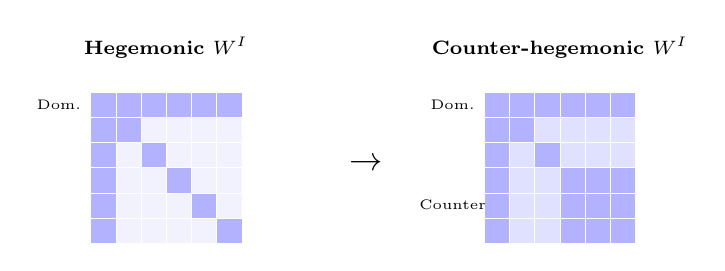
\begin{tikzpicture}[scale=1]
\def\N{6}
\def\s{0.32}

%% Hegemonic W^I: hub-spoke centered on dominant media
\node[font=\scriptsize\bfseries, above] at ({3*\s}, {\N*\s+0.3}) {Hegemonic $W^I$};
\foreach \i in {1,...,\N} {
  \foreach \j in {1,...,\N} {
    \pgfmathparse{
      (\i==1 && \j==1) ? 80 :
      (\i==1) ? 50 :
      (\j==1) ? 40 :
      (\i==\j) ? 30 :
      5
    }
    \edef\bp{\pgfmathresult}
    \fill[blue!\bp, draw=white, line width=0.08pt]
      ({(\j-1)*\s}, {(\N-\i)*\s}) rectangle +(\s,\s);
  }
}
\node[font=\tiny] at ({-0.4}, {5.5*\s}) {Dom.};

%% Arrow
\node[font=\large] at (3.5, 1.0) {$\to$};

%% Counter-hegemonic W^I: more distributed
\begin{scope}[xshift=5cm]
\node[font=\scriptsize\bfseries, above] at ({3*\s}, {\N*\s+0.3}) {Counter-hegemonic $W^I$};
\foreach \i in {1,...,\N} {
  \foreach \j in {1,...,\N} {
    \pgfmathparse{
      (\i==1 && \j==1) ? 45 :
      (\i==1) ? 20 :
      (\j==1) ? 15 :
      (\i==\j) ? 35 :
      (\i>=4 && \j>=4) ? 30 :
      12
    }
    \edef\bp{\pgfmathresult}
    \fill[blue!\bp, draw=white, line width=0.08pt]
      ({(\j-1)*\s}, {(\N-\i)*\s}) rectangle +(\s,\s);
  }
}
\node[font=\tiny] at ({-0.4}, {5.5*\s}) {Dom.};
\node[font=\tiny] at ({-0.4}, {1.5*\s}) {Counter};
\end{scope}
\end{tikzpicture}
\end{center}
\vspace{-0.5em}
\small Left: hegemonic $W^I$ --- hub-spoke, centered on the dominant coalition's media (column~1, attention paid to the dominant outlet, is bright). Right: counter-hegemonic $W^I$ --- the dominated agents (lower-right block) have formed their own information network. Row-normalizing the cell values (\texttt{code/ch24.py}): hegemonic $\pi_{\text{dom}} = 0.37$, $\Neff = 4.63$, $\Gamma = 0.72$; counter-hegemonic $\pi_{\text{dom}} = 0.15$, $\Neff = 5.88$, $\Gamma = 0.67$. Power concentration falls, as $\Neff$ shows. $\Gamma$ falls slightly too: a hub everyone listens to mixes \emph{fast}, so the hegemonic network is the better integrated one. $\Gamma$ measures integration, not concentration.
\end{vizpanel}


%% =====================================================================
\section{State Crisis as Hegemonic Collapse}
\label{ch24:sec:crisis}
%% =====================================================================

\begin{definition}[State Crisis]\label{ch24:def:crisis}
A \textbf{state crisis} occurs when the hegemonic equilibrium loses stability or ceases to exist: the three loops (production, information, solidarity) decouple, and the dominant coalition can no longer maintain consent. In the co-evolutionary dynamics (Chapter~13), this corresponds to the Jacobian $\mathcal{J}$ of the hegemonic fixed point acquiring an eigenvalue of modulus $\ge 1$; in the saddle-node of Proposition~\ref{ch24:thm:counter} the eigenvalue reaches $+1$ and the equilibrium disappears.
\end{definition}

This definition is the book's, not Skocpol's. \citet{skocpol1979states} is explicitly structural and non-voluntarist: social revolutions are not made by movements with new ideas but happen when international (military and fiscal) pressure breaks the administrative and coercive apparatus of agrarian-bureaucratic states, often because dominant classes block the reforms that would meet the pressure, and when agrarian structures give peasant communities the autonomy to revolt. Her theory concerns social revolutions within these scope conditions. Bolivia 1952 fits it far better than 2003, which was a crisis of government in a democracy.

\begin{conjecture}[Conditions for Hegemonic Collapse]\label{ch24:prop:collapse}
The hegemonic equilibrium loses stability when one or more of the following holds (the first two are Gramscian channels; the last two are Skocpol's):
\begin{enumerate}
\item \textbf{The counter-signal crosses the threshold}: the information network becomes too diverse ($\Neff^I$ rises) for the dominant coalition to control, and counter-hegemonic channels accumulate until $\mu\|\Delta(W^I\mathbf{r})\| > (1-\rho)s^*$ (Proposition~\ref{ch24:thm:counter}).

\item \textbf{An exogenous shock exposes the gap}: a crisis (financial, environmental, health) reveals the allocation inequality that the hegemonic $W^I$ had normalized. The shock changes the returns $\mathbf{r}_t$ dramatically, and the $W^I$-weighted signal shifts even under the existing information structure.

\item \textbf{State breakdown under external pressure} (Skocpol): international military or fiscal pressure strains the state, and dominant-class resistance to reform splits the elite and paralyzes the state's coercive and administrative capacity. In Chapter~14's terms: the $\{F, B\}$ coalition's feasibility set $\mathcal{F}(S)$ shrinks and some $B$ agents defect.

\item \textbf{Revolt from below enabled by structure} (Skocpol): agrarian or communal structures that give the dominated autonomous organization (peasant communities, unions) allow mass revolt once the state is weakened. In Chapter~14's terms: the alliance $\{M, W\}$ or $\{B, M, W\}$ becomes feasible.
\end{enumerate}
\end{conjecture}

\begin{example}[Bolivia 2000--2006: From Crisis to Counter-Hegemony]\label{ch24:ex:crisis}
The neoliberal hegemony collapsed through a sequence in which all four channels were present ($N_{\text{eff}}^I$ values are \illustrative):

\textbf{Condition 1}: Community radio and social movements created alternative $W^I$ channels throughout the 1990s. $N_{\text{eff}}^I$ rose from $\approx 2.0$ to $\approx 2.8$.

\textbf{Condition 2}: The Water War (2000) exposed the cost of privatization (sharp tariff increases). The shock changed $\mathbf{r}_t$: the ``returns to privatization'' signal turned negative for poor households.

\textbf{Condition 3}: Fiscal stress weakened the state: the 1999--2002 slowdown and a large fiscal deficit led to the IMF-backed income-tax proposal of February 2003, which provoked riots and a police mutiny in La Paz. The governing coalition split.

\textbf{Condition 4}: The Gas War (2003) formed a cross-class coalition from autonomous organizations: El Alto's \textit{juntas vecinales} (working class), rural cocaleros and campesino unions, and middle-class professionals united against gas export plans. The alliance $\{M, W\}$ forced President S\'{a}nchez de Lozada's resignation in October 2003; renewed protests forced President Mesa's resignation in June 2005.

The hegemonic equilibrium was unstable by 2003. The transition to the MAS hegemony (2006) was the co-evolutionary system settling into a new structural equilibrium --- with different ownership of and fiscal claims on $W^P$ (nationalized gas), different $W^I$ (state media + indigenous networks), and different $\boldsymbol{\theta}^*$ (indigenous identity, state-led development, plurinationalism). The change in $W^P$ was one of ownership and rent capture, not of production linkages: the integration of the domestic input-share network barely moved ($\Gamma = 0.518$ in 2006 and $0.504$ in 2009), and the hydrocarbons sector stayed at its periphery, with a Perron weight below 0.09 in every year of 2006--2009 (INE input--output matrices, base 1990, 12 sectors; author's calculations, \texttt{data/compute/compute\_bolivia\_io.py}; \citealp{ine2026sut}; Chapter~23).
\end{example}


%% =====================================================================
\section{The Hegemonic Cycle}
\label{ch24:sec:cycle}
%% =====================================================================

\begin{conjecture}[The Hegemonic Cycle]\label{ch24:thm:cycle}
In the co-evolutionary system with formation and coalition dynamics, the long-run trajectory exhibits a hegemonic cycle:
\begin{enumerate}
\item \textbf{Establishment}: A coalition wins and implements $\Delta W$ (production restructuring) + $\Delta W^I$ (narrative control). The new structure becomes a structural equilibrium. Consent is formed through $W^I$.
\item \textbf{Consolidation}: The hegemony stabilizes. Preferences converge to $\boldsymbol{\theta}^*$. Growth occurs within the structure. Inequality is accepted.
\item \textbf{Erosion}: $N_{\text{eff}}^I$ increases (new media, new movements). The formation signal diversifies. Peripheral agents begin to see alternative returns. $\Delta\theta$ begins.
\item \textbf{Crisis}: An exogenous shock or accumulated $\Delta W^I$ pushes preferences past the basin boundary. The hegemonic equilibrium becomes unstable. The dominant coalition fragments.
\item \textbf{Transition}: A new coalition forms and implements a new $\Delta W$. Return to step 1 with a different structure.
\end{enumerate}

The cycle period depends on: (a) the speed of $N_{\text{eff}}^I$ growth (faster media diversification = shorter cycle), (b) the persistence parameter $\rho$ (stickier preferences = longer consolidation phase), (c) the frequency of exogenous shocks (more shocks = more crisis triggers).
\end{conjecture}

\begin{remark}[What a cycle requires]\label{ch24:rem:cycle_mechanism}
This is a conjecture, not a theorem. A system whose fixed points are stable, driven by a monotonically rising $\Neff^I$, does not cycle: it moves once from one equilibrium to another and stays. A genuine cycle needs either recurring exogenous shocks or a slow feedback that reverses the drift. In model \eqref{ch24:eq:counter_model}, a hysteresis loop arises if the counter-signal $s$ drifts up slowly while the old hegemony rules (erosion), the system jumps at $s^*$ (crisis), and the new hegemony then uses its control of $W^I$ to push $s$ back down past the lower fold of the reversed model (consolidation of the new order). Writing down and estimating that slow equation is an open problem.
\end{remark}

\begin{intuition}[The Latin American hegemonic cycle]
The Latin American political cycle (Chapter~14's pendulum) is the hegemonic cycle operating at the regional scale:

\textbf{Oligarchic hegemony} (pre-1930): export agriculture and mining, $N_{\text{eff}}^I \approx 1$--2. Collapsed with the Great Depression (exogenous shock to $W^P_{\text{global}}$).

\textbf{National-populist hegemony} (1930--1960s): ISI, mass media controlled by the state, labor incorporation. Collapsed as the bourgeoisie defected (ISI success raised $\pi_B$, triggering alliance switch per Chapter~14).

\textbf{Bureaucratic-authoritarian hegemony} (1960s--1980s): military rule, controlled media ($N_{\text{eff}}^I$ suppressed by censorship), alliance $\{F, B, M\}$. Collapsed with the debt crisis (exogenous shock) and democratization.

\textbf{Neoliberal hegemony} (1985--2003): Washington Consensus, private media, $N_{\text{eff}}^I \approx 2$--3. Collapsed as social movements created alternative $W^I$.

\textbf{Left-populist hegemony} (2006--2019 in Bolivia): resource nationalism, state + indigenous media, $N_{\text{eff}}^I \approx 3$. Eroding as social media diversifies $W^I$.

The hegemonies lasted between about 13 and 40 years. The first three collapsed after exogenous shocks (the Depression, the debt crisis) or elite defection; the information channel was decisive mainly in the last two. If digital media keep adding channels faster than any coalition can control them, the cycle may be accelerating --- a hypothesis that five episodes cannot test (Exercise~24.6), and one that depends on whether platforms raise or lower $\Neff^I$ (Chapter~27).
\end{intuition}


%% =====================================================================
\section{Summary}
\label{ch24:sec:summary}
%% =====================================================================

\begin{enumerate}
\item \textbf{Hegemony} is a structural equilibrium where the dominant coalition's preferred $W$ is sustained by $W^I$-formed preferences that consent to it (the consent half of Gramsci's ``consent armoured by coercion''). Three conditions: power concentration ($\Neff^P \ll N$), consent, formation alignment. Three reinforcing loops ($W^P$, $W^I$, $W^U$) make it stable.

\item The \textbf{maintenance cost} of hegemony rises with $\Neff^I$ (more independent weight to counter) and falls when $W^I$ is weakly coupled ($1-\lambda_2$ small: the consensus is cheap for anyone to move). Concentration is measured by $\Neff^I$, never by $\Gamma^I$: a hub everyone listens to has a large $\Gamma$.

\item \textbf{Counter-hegemony} is $\Delta W^I$. Under conformity, it succeeds by a shock that carries preferences past the separatrix, or by a persistent signal above the saddle-node threshold, $\mu\|\Delta(W^I\mathbf{r})\| > (1-\rho)s^*$.

\item \textbf{State crisis} combines Gramscian channels (counter-signals, shocks that expose inequality) with Skocpol's structural ones (state breakdown under external pressure, revolt enabled by autonomous organization). Bolivia 1952 fits Skocpol's scope; 2000--2005 was a crisis of government.

\item The \textbf{hegemonic cycle} (establishment $\to$ consolidation $\to$ erosion $\to$ crisis $\to$ transition) is a conjecture: it requires recurring shocks or a slow reversing feedback, which remains to be modelled and estimated.
\end{enumerate}


%% =====================================================================
\section{Exercises}
\label{ch24:sec:exercises}
%% =====================================================================

\begin{enumerate}[label=\textbf{24.\arabic*}, leftmargin=3em]

\item \textbf{Hegemony as fixed point.} For a 2-group economy (Elite $E$, Masses $M$): write the co-evolutionary system (Chapter~13) with $W^I$ controlled by $E$. Find parameter values under which a fixed point of this system satisfies all three conditions of Definition~\ref{ch24:def:hegemony}, and is therefore a hegemonic equilibrium (Definition~\ref{ch24:thm:hegemony}; that definition holds by construction, so the work is in finding the fixed point and checking the conditions). Under what parameter values does a counter-hegemonic equilibrium also exist?

\item \textbf{Maintenance cost.} For Bolivia's MAS hegemony (2006--2019): estimate the cost of $W^I$ control (state media budget, community communication spending). How does it compare with the government's total budget? At what $N_{\text{eff}}^I$ does the cost exceed the coalition's willingness to pay?

\item \textbf{Counter-hegemony simulation.} Start from a hegemonic equilibrium. Add counter-hegemonic $\Delta W^I$ edges incrementally ($\Delta\lambda^I = +0.02$ per period). Simulate 50 periods. At what period does the hegemonic equilibrium collapse? How does this depend on $\rho$?

\item \textbf{Bolivia's hegemonic transitions.} Map all five hegemonies from the Prebisch Connection box to the structural power game (Chapter~14): for each, identify the coalition, the $W^I$ control mechanism, the $N_{\text{eff}}^I$, and the trigger for collapse.

\item \textbf{Skocpol's conditions.} For the 2000--2006 Bolivian transition: verify each of the four conditions in Conjecture~\ref{ch24:prop:collapse}. Which was the binding condition? Could the neoliberal hegemony have survived if any one condition had not been met?

\item \textbf{The acceleration of the cycle.} Plot the duration of each Latin American hegemonic epoch (from the Prebisch Connection box) against $N_{\text{eff}}^I$. Is there a negative correlation (more information diversity = shorter hegemonic periods)? What does this predict for the current period?

\item \textbf{Gramsci vs.\ Skocpol.} Gramsci emphasized consent (the formation of preferences). Skocpol emphasized structural conditions (fiscal crisis, military defeat, elite splits). In the model: Gramsci's hegemony is the $W^I$ loop (preference formation); Skocpol's crisis is the $W^P$ loop (economic disruption) + the coalition loop (elite defection). Are these complementary or competing? Under what parameter values does each mechanism dominate?
\end{enumerate}


%% =====================================================================
\newpage
\section*{Mathematical Appendices}
\addcontentsline{toc}{section}{Mathematical Appendices}
%% =====================================================================


\subsection*{Appendix 24A: Stability of the Hegemonic Equilibrium}
\addcontentsline{toc}{subsection}{Appendix 24A: Stability Analysis}
\label{ch24:app:stability}

\paragraph{The hegemonic fixed point.} Let $(W^*, \boldsymbol{\theta}^*, \x^*)$ be a hegemonic equilibrium. The stability is governed by the eigenvalues of the co-evolutionary Jacobian (Chapter~13, Appendix~13B):
\begin{equation}
\mathcal{J} = \begin{pmatrix} \partial T/\partial\boldsymbol{\theta} & \partial T/\partial W \\ \partial\mathcal{E}/\partial\boldsymbol{\theta} & \partial\mathcal{E}/\partial W \end{pmatrix}.
\end{equation}

The hegemony is stable if $\rho(\mathcal{J}) < 1$. It loses stability when:
\begin{enumerate}
\item The formation feedback is too strong: $\rho(J) \to 1$, where $J = \rho I + \mu\phi W^I C P$ is the formation Jacobian (Proposition~\ref{ch10:prop:jacobian}). This may occur as counter-hegemonic channels strengthen the conformity feedback; in the scalar model \eqref{ch24:eq:counter_model} the relevant eigenvalue is $\rho + (1-\rho)g'(\theta_h)$, which reaches 1 exactly at the saddle-node.
\item An exogenous shock changes the returns $\mathbf{r}$ suddenly, shifting the formation map $T$ and moving the system outside the basin of attraction.
\item The coalition dynamics (Chapter~14) produce an alliance switch that changes $W$ discretely.
\end{enumerate}

\paragraph{Bifurcation.} The relevant bifurcation is a \textbf{saddle-node} (fold), not a pitchfork. In model \eqref{ch24:eq:counter_model}, as the counter-signal $s$ rises the stable hegemonic fixed point and the unstable separatrix approach each other, merge at $s^*$ ($s^* = 0.181$ for $\beta = 10$; \texttt{code/ch24.py}) and vanish. Below $s^*$: two stable equilibria (hegemony and counter-hegemony) separated by the separatrix, so a large enough shock can push the system across. Above $s^*$: only the counter-hegemonic equilibrium survives. Running $s$ back down does not restore the old hegemony until a second fold is reached, at $s = -s^*$ (a pro-hegemonic signal; by the symmetry of $g$): hysteresis, which is why hegemonic transitions are not reversed by small reversals of the signal.


\subsection*{Appendix 24B: Gramsci's Categories in Matrix Notation}
\addcontentsline{toc}{subsection}{Appendix 24B: Gramsci in Matrix Notation}
\label{ch24:app:gramsci}

\paragraph{Hegemony.} A structural equilibrium where the dominant group's power ($\boldsymbol{\pi}$) is reproduced by $W^I$-formed consent ($\boldsymbol{\theta}^*$). For Gramsci consent never stands alone: it is ``armoured by coercion'', and the state is political society plus civil society. The model captures the consent half; coercion is the coalition's reserve option.

\paragraph{Historic bloc.} The alignment of a social coalition, its economic base and its worldview into a durable unit. In this chapter: the triple alignment of loops 1--3 (production, information, solidarity) around one coalition. The formalization is ours; Gramsci's concept is broader.

\paragraph{Passive revolution.} Transformation directed from above that absorbs the leaders and demands of subaltern groups without their autonomous mobilization: in Gramsci's phrase, a ``revolution-restoration''. It is arguably the Gramscian concept most used for Latin America. In this chapter: a $\Delta W$ implemented by the dominant coalition that co-opts the counter-hegemonic channels, moving $\boldsymbol{\theta}$ toward consent before $s$ reaches $s^*$.

\paragraph{Organic intellectuals.} For Gramsci, intellectuals tied organically to a class --- including subaltern classes --- who give it homogeneity and awareness of its function; they are defined by that tie, not by audience size. In this chapter: the agents, on either side, whose position in $W^I$ lets them shape a class's formation signal. When they belong to the dominant coalition they hold high $\pi^I_j$, and in Chapter~8's terms they are the DeGroot influencers whose beliefs weigh most in the consensus.

\paragraph{War of position.} The slow process of building alternative $W^I$ channels (counter-hegemonic institutions: schools, media, unions, parties). In this chapter: the gradual increase of $N_{\text{eff}}^I$ through new information edges. The ``war of position'' IS the accumulation of $\Delta W^I$ over time.

\paragraph{War of maneuver.} The rapid seizure of state power once the counter-hegemonic movement has sufficient support. In this chapter: the moment when preferences cross the basin boundary and the demand for structural change becomes politically irresistible. The ``war of maneuver'' IS the coalition switch (Chapter~14) triggered by the preference shift.

\paragraph{Interregnum.} The period between the collapse of one hegemony and the establishment of the next: ``the old is dying and the new cannot be born'' (Q3 \S34). In this chapter: the co-evolutionary system is between structural equilibria. $W^I$ is contested; $\boldsymbol{\theta}$ is in flux; $W^P$ is unstable. This is the period of maximum vulnerability --- of Gramsci's ``morbid symptoms'' (political instability, democratic backsliding, authoritarianism).


%% =====================================================================
\subsection*{Structuralist Case Study: Gramsci and Skocpol on Structural Crisis}
\addcontentsline{toc}{subsection}{Structuralist Case Study: Gramsci and Skocpol}
%% =====================================================================

Antonio Gramsci (1891--1937) and Theda Skocpol (b.\ 1947) represent two approaches to the same question: why do structures of domination persist, and how do they collapse? Gramsci emphasized consent and cultural production. Skocpol emphasized structural conditions and state capacity. This chapter argues that both are correct about different loops of the same co-evolutionary system.

\textbf{Gramsci: hegemony as formation.} Gramsci, writing from Mussolini's prison, asked why the Italian working class accepted capitalist domination even when it was materially disadvantaged. His answer: hegemony --- the process by which the dominant class's worldview becomes the ``common sense'' of society. In this book's notation: hegemony is the steady state of the formation model where $W^I$ produces preferences that consent to the $W^P$-determined allocation. Gramsci's ``common sense'' is $\boldsymbol{\theta}^*$; the formative position of his organic intellectuals is a position in $W^I$; his ``war of position'' is the accumulation of counter-hegemonic $\Delta W^I$.

This is a formal reinterpretation, and Gramsci would resist parts of it. The mechanism of Chapters~8--10 --- ideas produced by specific agents, disseminated through specific channels (media, schools, churches = $W^I$ edges), and internalized as preferences --- captures the consent side of his concept. It leaves out coercion (hegemony is ``armoured by coercion''), the historic bloc that welds an economic base to a worldview, and passive revolution, the reorganization from above that absorbs subaltern demands (Appendix~24B). The information structure is the part of hegemony the model can see.

\textbf{Skocpol: crisis as structural breakdown.} Skocpol, analyzing the French, Russian, and Chinese revolutions, argued against voluntarist explanations, borrowing Wendell Phillips's line that ``revolutions are not made; they come.''
% TODO-VERIFY: page of the Phillips quotation in Skocpol (1979), ch. 1.
 Social revolutions occurred when international military and fiscal competition broke the administrative and coercive apparatus of agrarian-bureaucratic old regimes --- often because landed dominant classes blocked the reforms that would have met the pressure --- and when agrarian structures gave peasant communities the solidarity and autonomy to revolt. Ideas and movements are, in her account, not the cause. In this chapter's notation: state crisis is the co-evolutionary system losing stability because the dominant coalition's resource base ($W^P$ position, $\mathcal{F}(S)$) collapses under external pressure and its members split, while the structure of $W^U$ among the dominated (communal solidarity) makes revolt feasible.

The mapping: international pressure = an exogenous shock to the global $W^P$ and to the fiscal capacity of the state (shrinking $\mathcal{F}(S)$). Dominant-class obstruction of reform = $B$ and $F$ refusing the $\Delta W$ that would meet the shock, and splitting over it (Chapter~14). Peasant revolt = autonomous organization of the dominated (high within-group $W^U$) once the state is weakened. The information channel, central for Gramsci, plays no causal role in Skocpol; this chapter's Conjecture~\ref{ch24:prop:collapse} combines the two, which is our synthesis, not hers. Her scope conditions fit Bolivia 1952 far better than the 2003--2005 crisis of government.

\textbf{The synthesis.} Gramsci explains why structures persist (the formation loop produces consent). Skocpol explains when they collapse (structural conditions destabilize the fixed point). Both are needed: without Gramsci, we cannot explain why the dominated accept the structure during ``normal'' times. Without Skocpol, we cannot explain the timing of crises. The co-evolutionary system offers a way to combine them: hegemony as a stable fixed point (Gramsci's consent), crisis as its loss of stability (driven, on Skocpol's account, by external pressure on the state rather than by ideas).

\begin{center}
\begin{tabularx}{\textwidth}{LLL}
\toprule
\textbf{Concept} & \textbf{Gramsci} & \textbf{Skocpol} \\
\midrule
Central question & Why do the dominated consent? & When does the state collapse? \\
Mechanism & $W^I$ forms preferences (consent, armoured by coercion) & External pressure breaks the state; agrarian structure enables revolt \\
Formal object & Hegemonic equilibrium (Def.~\ref{ch24:thm:hegemony}) & Stability loss (Conj.~\ref{ch24:prop:collapse}) \\
Time horizon & Long-run (generations) & Medium-run (decades) \\
Policy variable & $\Delta W^I$ (counter-hegemony) & Exogenous shock + coalition \\
Bolivia application & MAS narrative control & 1952 revolution (best fit) \\
\bottomrule
\end{tabularx}
\end{center}

Gramsci wrote from prison. Skocpol wrote from Harvard. Between them, they describe the two phases of structural politics: the long war of position (building alternative $W^I$) and the sudden war of maneuver (the crisis that topples the structure). The co-evolutionary system of this book is one way to put both in a single dynamical model.


%% =====================================================================
\subsection*{Further Reading}
\addcontentsline{toc}{subsection}{Further Reading}
%% =====================================================================

\textbf{Gramsci:} \citet{gramsci1971selections}, \textit{Selections from the Prison Notebooks}, edited by Q.\ Hoare and G.\ N.\ Smith. For the Latin American reception: \citet{portantiero1981usos}, \textit{Los usos de Gramsci}. For the application to media: \citet{hall1986gramsci}, ``Gramsci's Relevance for the Study of Race and Ethnicity.''

\textbf{Skocpol:} \citet{skocpol1979states}, \textit{States and Social Revolutions: A Comparative Analysis of France, Russia, and China}. For the extension to the ``third wave'': \citet{goodwin2001no}, \textit{No Other Way Out: States and Revolutionary Movements}.

\textbf{Hegemony and development:} \citet{cox1983gramsci}, ``Gramsci, Hegemony and International Relations.'' \citet{laclau1985hegemony}, \textit{Hegemony and Socialist Strategy}. For Bolivia specifically: \citet{garcialinera2008potencia}, \textit{La potencia plebeya}.

\textbf{Information and political change:} \citet{enikolopov2011media}, ``Media and Political Persuasion.'' \citet{kern2009opium}, ``Opium for the Masses.'' \citet{manacorda2020liberation}, ``Liberation Technology: Mobile Phones and Political Mobilization in Africa.''

\end{document}
